% Template LaTeX file for DAFx-19 papers
%
% To generate the correct references using BibTeX, run
%     latex, bibtex, latex, latex
% modified...
% - from DAFx-00 to DAFx-02 by Florian Keiler, 2002-07-08
% - from DAFx-02 to DAFx-03 by Gianpaolo Evangelista
% - from DAFx-05 to DAFx-06 by Vincent Verfaille, 2006-02-05
% - from DAFx-06 to DAFx-07 by Vincent Verfaille, 2007-01-05
%                          and Sylvain Marchand, 2007-01-31
% - from DAFx-07 to DAFx-08 by Henri Penttinen, 2007-12-12
%                          and Jyri Pakarinen 2008-01-28
% - from DAFx-08 to DAFx-09 by Giorgio Prandi, Fabio Antonacci 2008-10-03
% - from DAFx-09 to DAFx-10 by Hannes Pomberger 2010-02-01
% - from DAFx-10 to DAFx-12 by Jez Wells 2011
% - from DAFx-12 to DAFx-14 by Sascha Disch 2013
% - from DAFx-15 to DAFx-16 by Pavel Rajmic 2015
% - from DAFx-16 to DAFx-17 by Brian Hamilton 2016
% - from DAFx-18 to DAFx-19 by Dave Moffat 2019
%
% Template with hyper-references (links) active after conversion to pdf
% (with the distiller) or if compiled with pdflatex.
%
% 20060205: added package 'hypcap' to correct hyperlinks to figures and tables
%                      use of \papertitle and \paperauthorA, etc for same title in PDF and Metadata
%
% 1) Please compile using latex or pdflatex.
% 2) If using pdflatex, you need your figures in a file format other than eps! e.g. png or jpg is working
% 3) Please use "paperftitle" and "pdfauthor" definitions below

%------------------------------------------------------------------------------------------
%  !  !  !  !  !  !  !  !  !  !  !  ! user defined variables  !  !  !  !  !  !  !  !  !  !  !  !  !  !
% Please use these commands to define title and author(s) of the paper:
\def\papertitle{notGuitar: A Real-Time Timbral Conversion System}
\def\paperauthorA{Jatin Chowdhury}
\def\paperauthorB{Paul Chyz}
\def\paperauthorC{Joey Hall}

% Authors' affiliations have to be set below

%------------------------------------------------------------------------------------------
\documentclass[twoside,a4paper]{article}
\usepackage{dafx_19}
\usepackage{amsmath,amssymb,amsfonts,amsthm}
\usepackage{euscript}
\usepackage[latin1]{inputenc}
\usepackage[T1]{fontenc}
\usepackage{ifpdf}

\usepackage[english]{babel}
\usepackage{caption}
\usepackage{subfig} % or can use subcaption package
\usepackage{color}

\setcounter{page}{1}
\ninept

\usepackage{times}
% Saves a lot of ouptut space in PDF... after conversion with the distiller
% Delete if you cannot get PS fonts working on your system.

% pdf-tex settings: detect automatically if run by latex or pdflatex
\newif\ifpdf
\ifx\pdfoutput\relax
\else
   \ifcase\pdfoutput
      \pdffalse
   \else
      \pdftrue
\fi

\ifpdf % compiling with pdflatex
  \usepackage[pdftex,
    pdftitle={\papertitle},
    pdfauthor={\paperauthorA, \paperauthorB, \paperauthorC},
    colorlinks=false, % links are activated as colror boxes instead of color text
    bookmarksnumbered, % use section numbers with bookmarks
    pdfstartview=XYZ % start with zoom=100% instead of full screen; especially useful if working with a big screen :-)
  ]{hyperref}
  \pdfcompresslevel=9
  \usepackage[pdftex]{graphicx}
  \usepackage[figure,table]{hypcap}
\else % compiling with latex
  \usepackage[dvips]{epsfig,graphicx}
  \usepackage[dvips,
    colorlinks=false, % no color links
    bookmarksnumbered, % use section numbers with bookmarks
    pdfstartview=XYZ % start with zoom=100% instead of full screen
  ]{hyperref}
  % hyperrefs are active in the pdf file after conversion
  \usepackage[figure,table]{hypcap}
\fi
\usepackage{cleveref}

\title{\papertitle}


\threeaffiliations{
\paperauthorA \,}
{\href{http://ccrma.stanford.edu}{Center for Computer Research in Music and Acoustics} \\ Stanford University \\ Palo Alto, CA \\ {\tt \href{mailto:jatin@ccrma.stanford.edu}{jatin@ccrma.stanford.edu}}}
{\paperauthorB \,}
{\href{https://minghsiehee.usc.edu/}{Ming Hsieh Department of Electrical Engineering} \\ University of Southern California \\ Los Angeles, CA }
{\paperauthorC \,}
{\href{https://minghsiehee.usc.edu/}{Ming Hsieh Department of Electrical Engineering} \\ University of Southern California \\ Los Angeles, CA }

\begin{document}
% more pdf-tex settings:
\ifpdf % used graphic file format for pdflatex
  \DeclareGraphicsExtensions{.png,.jpg,.pdf}
\else  % used graphic file format for latex
  \DeclareGraphicsExtensions{.eps}
\fi

\maketitle
\section{Abstract}
NotGuitar is a DSP system designed to perform real-time timbral conversion from electric guitar to saxophone.
In order to preserve the dynamic and expressive elements of the guitarist's playing as much as possible,
notGuitar does not use MIDI or synthesis, but simply processes the input guitar signal. 
NotGuitar was implemented using a Texas Instruments DSK6713 DSP board in May 2018 at the University of
Southern California.

\section{Introduction}
The specific sound of a particular instrument, or ``timbre'', is made up primarily of two parts: frequency characteristics
(harmonic structure) and an amplitude characteristics (attack, sustain, release)
\cite{Zolzer:2011:DDA:2028616}. NotGuitar uses note onset and envelope detection combined with
amplitude envelope modulation to alter the amplitude characteristics.
To affect the frequency characteristics, notGuitar uses a Sliding Discrete Fourier Transform (SDFT)
to perform rough pitch detection, then uses the rough pitch detection
to inform an adaptive circular convolution filter.
The full system architecture can be seen in Fig. \ref{flowchart}.

\begin{figure*}[ht]
  \center
  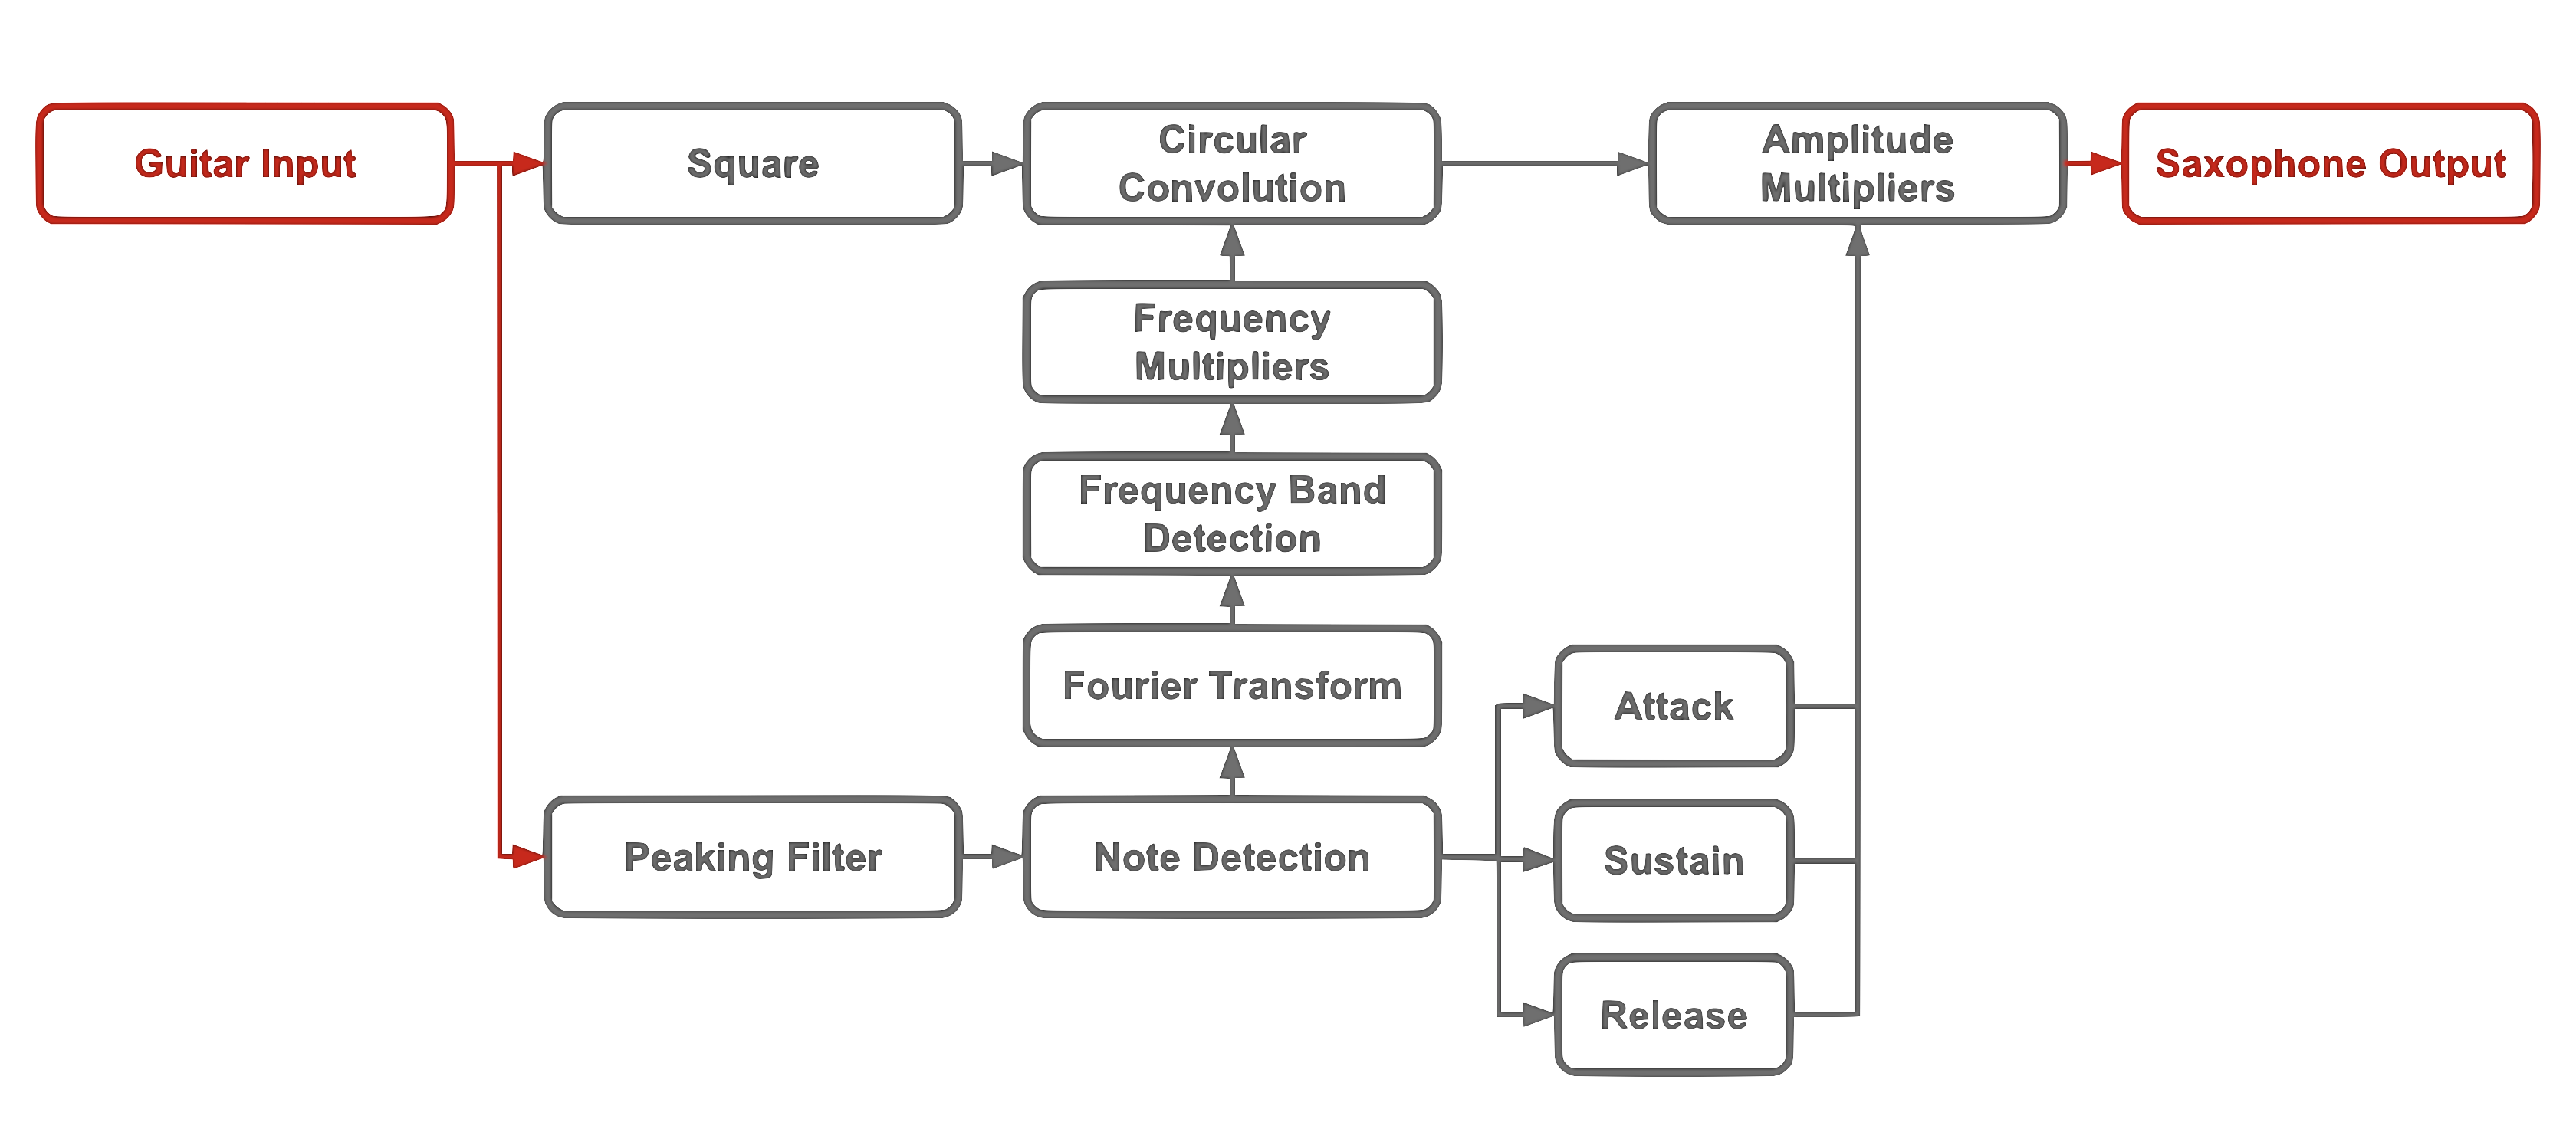
\includegraphics[width=5in]{Pictures/FlowChart.png}
  \caption{\label{flowchart}{\it notGuitar System Flowchart}}
  \end{figure*}

\section{Frequency Characteristics}
The frequency component of an instrument's timbre is typically referred to as the instrument's
``harmonic structure.'' Essentially, any note played on any instrument produces sound not just at the 
fundamental frequency of that note, but also at every multiple of that frequency, known as ``overtones.''
The frequency characteristic of individual instruments exists because the relative amplitude of each harmonic is different for each instrument.
\newline\newline
Our plan for manipulating the frequency content of the signal was to split our frequency spectrum linearly, 
with enough resolution to isolate individual overtones of any guitar note. We would then use guitar and saxophone 
sample recordings to train sets of multipliers that could act on the frequency bands to transform the harmonic structure 
of the guitar to that of the saxophone. Additionally, by detecting a rough frequency band that contained the fundamental, 
we could tune our multipliers to more accurately represent the harmonic structure relative to the fundamental frequency of the input signal.

\subsection{Different Approaches}
Our approach towards the frequency component of the guitar to saxophone timbral shift went through many iterations which will be outlined below:

\subsubsection{Sub-banding Filter Bank}
We initially decided to use a linear sub-banding filter bank to split the signal
into linearly spaced frequency bands, detect which of the sub-bands contained the
fundamental frequency, apply the corresponding set of multipliers, and then sum
the signal back together for the output. We abandoned this approach due to the difficulty
of summing the sub-bands back together. Since each sub-band would have it's own group delay
and phase delay, summing the bands correctly would have been non-trivial.

\subsubsection{Short Time Fourier Transform}
Our next plan was to use a Short Time Fourier Transform (STFT) to split
up the frequency spectrum. Since an N-window Fourier Transform essentially splits
the positive frequencies into N linearly spaced frequency bins, we could use the STFT
to find the fundamental frequency, then apply the multipliers, and use an inverse STFT
to bring the signal back to the time domain. While this method was well
suited for our purposes, we ended up abandoning the STFT after finding other methods
with lower time complexity.

\subsubsection{Sliding Discrete Fourier Transform}
In the system described above, the STFT would be operating on nearly identical
windows in consecutive time steps. The only differences would be one new sample
entering the window, one old sample leaving the window, and all the other samples
being shifted one sample over. Using this information, we next considered using a
Sliding Discrete Fourier Transform (SDFT) \cite{SDFT}. While the STFT has a time complexity
of $\mathcal{O}(n\log{}n)$ for both the forward and inverse transforms,
the SDFT is $\mathcal{O}(n)$ for the forward transform. In the final system, the SDFT is used to calculate the
Fourier Transform of the first four frequency bins, which then informs the system which set
of frequency multipliers to use for circular convolution.

\subsubsection{Circular Convolution}
Since the multiplication of two signals in the frequency domain
corresponds to the convolution of those signals in the time domain,
we ultimately decided to use circular convolution to implement the
filters in our system. The SDFT needs N complex-by-complex multiplications
for the forward transform, and $\frac{N}{2}$ real-by-complex multiplications
for the inverse transform. With an additional N real-by-complex multiplications
for the frequency multipliers, the total time complexity of the system coumes out to
$\mathcal{O}(7n)$. By contrast, circular convolution needs only N real-by-real
multiplications, for a total time complexity $\mathcal{O}(n)$.

\subsection{Frequency Multipliers}
After making the decision to use circular convolution for frequency filtering, we needed to generate
the overtone weightings to properly convert a guitar's harmonic
structure into one that matches a saxophone. To do this, we recorded
25 notes on both guitar and saxophone, and used \texttt{Matlab} to detect the
relative amplitudes of each overtone for each note. These relative
amplitudes allowed us to calculate a multiplier value to be applied to
each overtone, imposing the frequency characteristics of a saxophone on
the guitar signal. However, our implementation of these frequency multipliers
needed to address limitations in frequency resolution, high frequency content,
and circular convolution adaptations.

\subsubsection{Frequency Resolution}
Due to the use of circular convolution to split the frequency spectrum
linearly, there were inherent limits on the width of each resulting frequency
bin. In order to maintain an acceptable resolution for the frequency multipliers,
we designed the convolution (as well as the SDFT used for pitch detection) to use frequency bins that are 128 Hz wide. This
width corresponds to the frequency spacing of the overtones for the lowest note
in our training system. As the input signal increases in frequency from that note,
the overtone spacing will increase, and the effective resolution of the system will
improve from its baseline accuracy. This fixed bin width also required a change from
our initial plan to isolate each overtone. Instead, we generated one set of frequency
multipliers for each frequency bin, averaged from the training notes with fundamental
frequencies in that bin. These averaged multipliers contained between 5 and 12 notes
per frequency bin. A backup set of multipliers was generated from the average of all 25
notes, to be used in case the SDFT was unable to detect the fundamental frequency.

\subsubsection{High Frequency Content}
During our frequency multiplier testing, we noted that the guitar spectrum
contained fewer high frequencies than the saxophone spectrum we were trying to
replicate. Since we wanted to avoid any synthesis or
sampling, we alterred our system so that instead of filtering the direct input signal
we filtered the input signal summed with a scaled square of itself. The scaling
allowed us to control the intensity of the high frequencies from the square relative
to the lower frequencies that were already present. By training with this modified signal
and performing the same operation on the input signal in our real-time system, we were able
to generate enough high frequency content and weight it appropriately to match the harmonic
structure of a saxophone.

\subsubsection{Final Adaptations}
Since we had originally planned to perform a DFT and an inverse DFT,
we had generated frequency weighting coefficients in the frequency domain.
After switching to a circular convolution filter however, we needed the weighting
coefficients to resemble a time domain signal that could be convolved in the time domain
with the input signal. To make this adjustment, we took the inverse DFT of the
weighting coefficients. In testing, we found that the SDFT was unable to accurately
detect the fundamental frequency during the attack and release parts of the envelope
(which makes sense, since these are relatively broad-band events), so we generated
a set of coefficients averaged over all 25 training notes to be used during these parts of the envelope.

\subsection{Training Process}
The process of generating frequency weighting coefficients can be seen in \Cref{freq1,freq2,freq3}.

\begin{figure*}[htpb]
  \center
  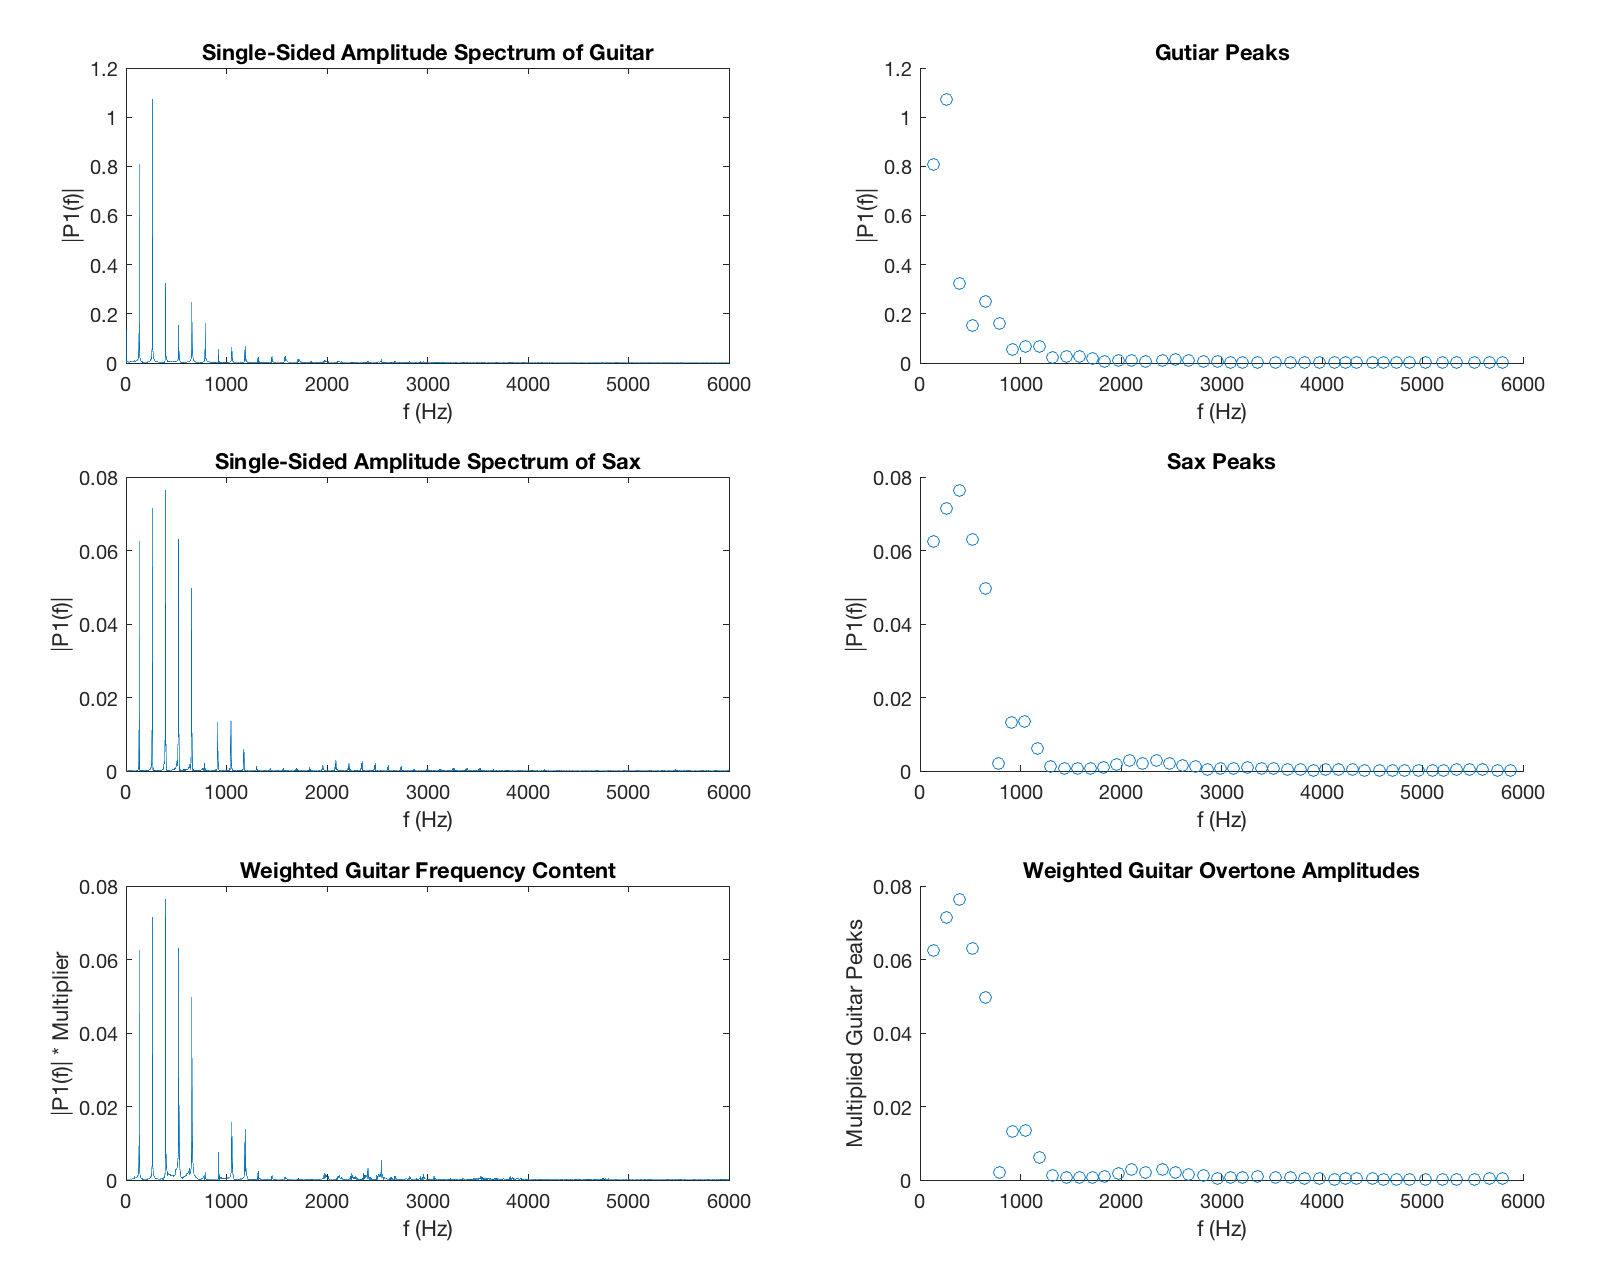
\includegraphics[width=7in]{Pictures/FreqPlot1.png}
  \caption{\label{freq1} {\it Overtone Amplitude Detection and Simulation of Applied Multipliers}}
  \end{figure*}

\begin{figure*}[ht]
  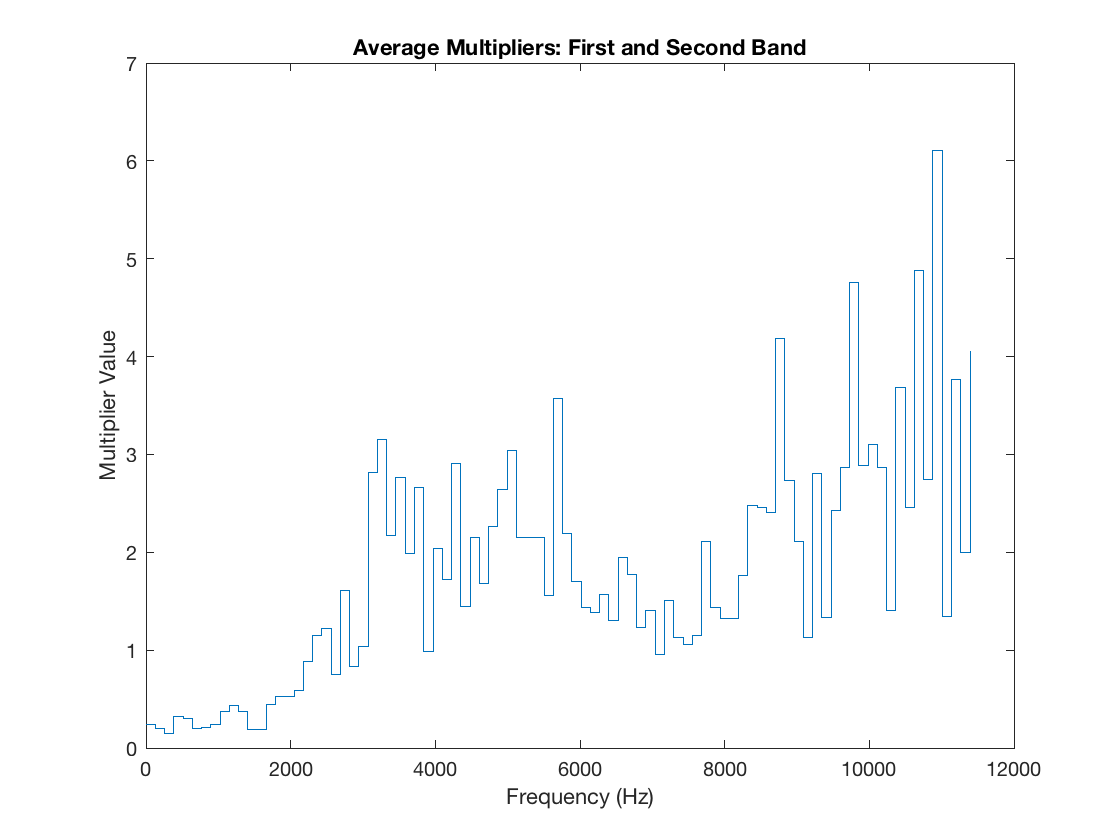
\includegraphics[width=3.5in]{Pictures/FreqMult1_2.png}
  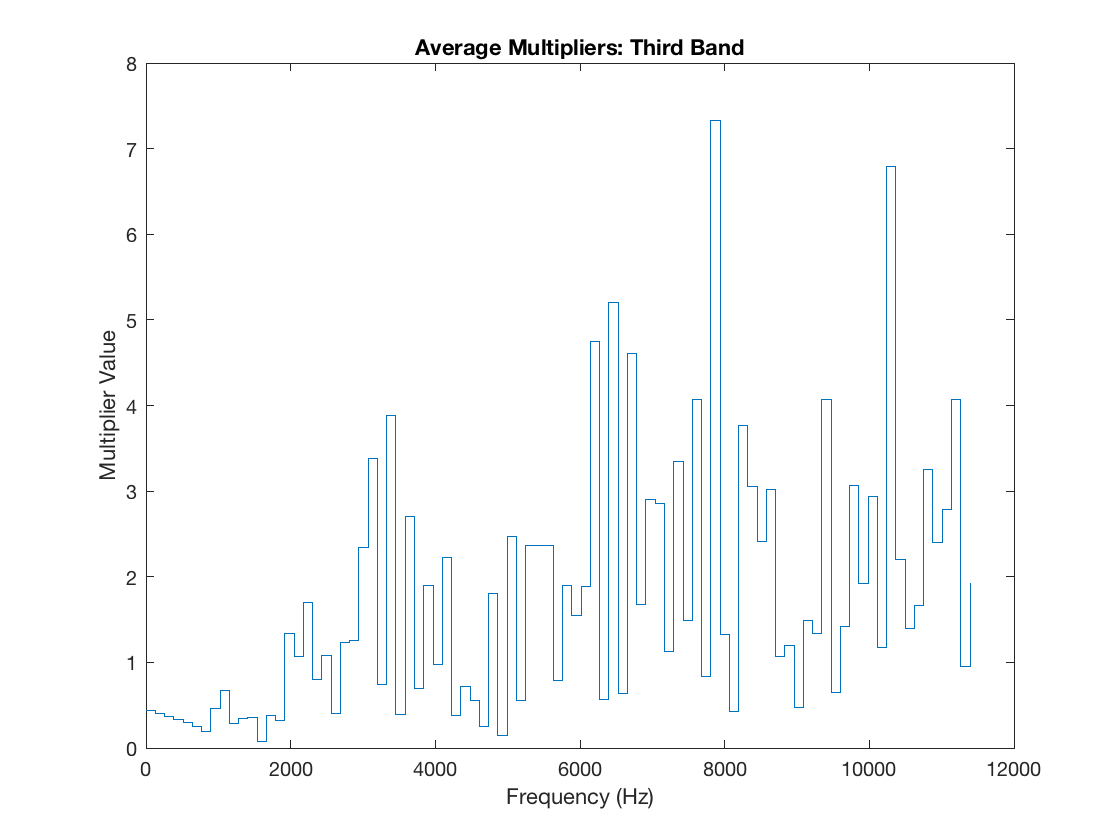
\includegraphics[width=3.5in]{Pictures/FreqMult3.png}
  \caption{\label{freq2} {\it Frequency Multipliers for the first and second frequency bin (left) and for the third frequency bin (right)}}
  \centering
  \end{figure*}

\begin{figure*}[ht]
  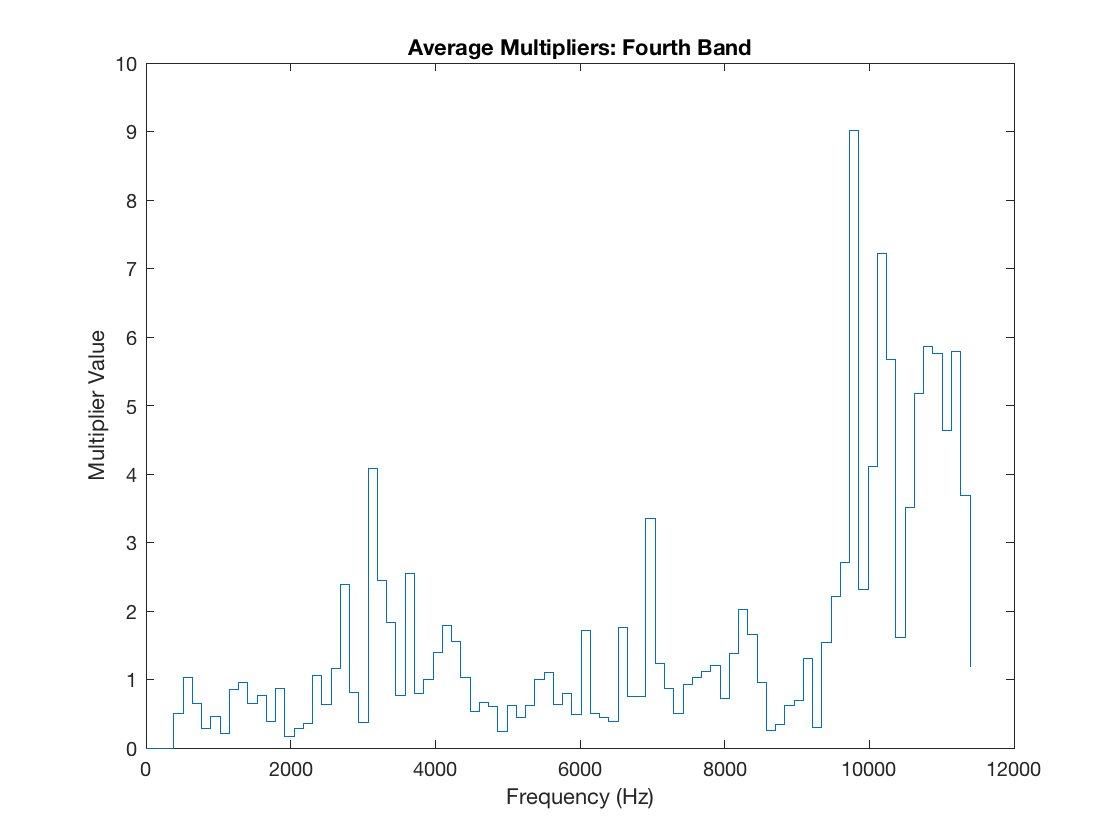
\includegraphics[width=3.5in]{Pictures/FreqMult4.png}
  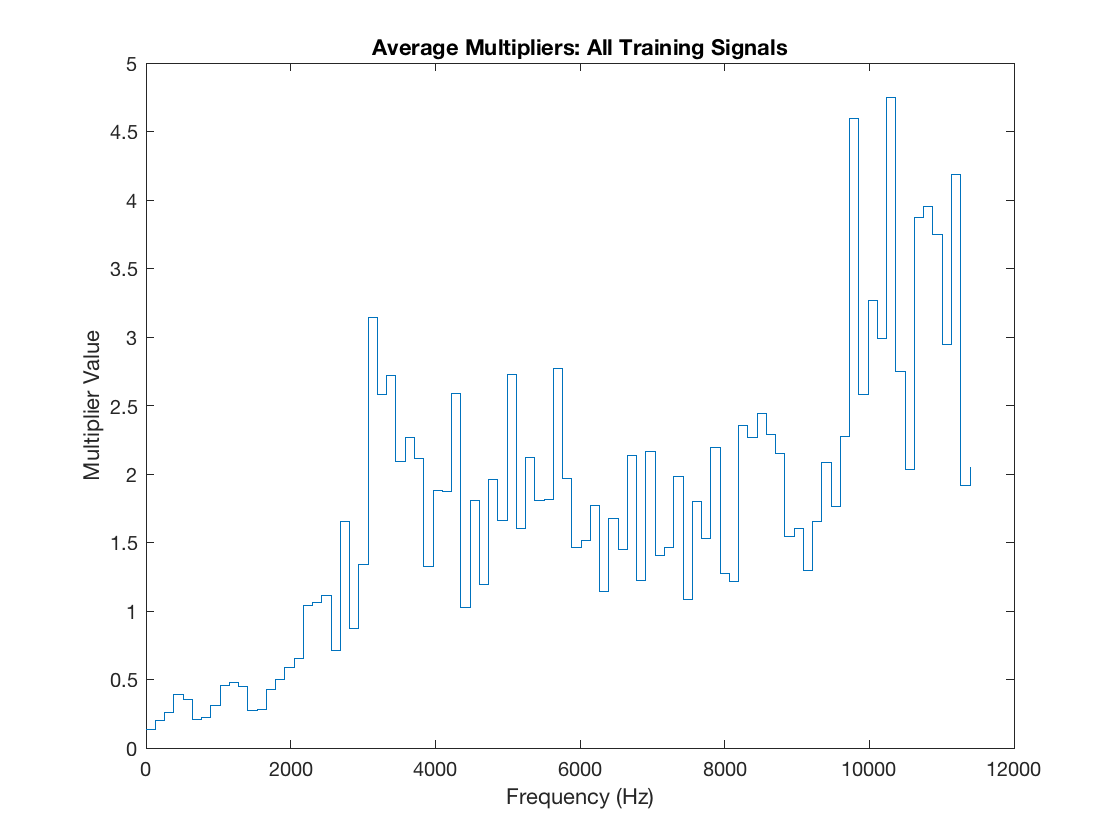
\includegraphics[width=3.5in]{Pictures/FreqMultAll.png}
  \caption{\label{freq3} {\it Frequency Multipliers for the fourth frequency bin (left) and for all training signals (right)}}
  \centering
  \end{figure*}


\subsection {Results}
The task of manipulating overtones with filtering was difficult
mainly due to the limitations of our real-time system, as well as
the frequency content (or lack thereof) of the guitar. Given those
limitations, the system performs well, and the output signal comes fairly
close to that of a saxophone. The main limitation of our real-time system
was that in order to complete all the neccesary processing without introducing
distortion from dropped samples, we needed to lower the sampling rate to 24 kHz.
Additionally, the lack of high frequency content in the
guitar signal made it difficult to produce a fully natural sound
as taking the square of the input signal introduced some high frequency
noise and distortion, that seemed to distract from the intended sound.
When paired with the amplitude modulation part of the system, the output
can resemble a saxophone, though with a slight dependence on playing
style (e.g. picking with fingers sounds better than picking with a pick).
\newline\newline
Some improvements that could be made to this system include more rigorous training, optimization of
frequency bin widths and average multipliers, and hardware improvements.
Training the multipliers with multiple versions of each note from different
guitars would produce a more robust system that would sound good
on many types of guitars. Similarly, optimizing the system to increase the
frequency resolution would allow for more isolated overtone multipliers.
This in turn would improve the effectiveness of the averaged multipliers.
Finally, using a more modern DSP board would allow us to increase the sample rate,
bringing us closer to the industry standard for audio technology, and allowing some of the noise
and distortion from the squared signal to be separated from the input signal
due to the increased frequency spectrum before the Nyquist frequency.

\color{black}
\section{Amplitude Characteristics}
Along with a unique harmonic structure, each musical instrument
also has a unique amplitude envelope, helping give it a unique timbre.
The amplitude envelope has three parts: the attack, sustain and release. 

%\begin{figure}[ht]
%  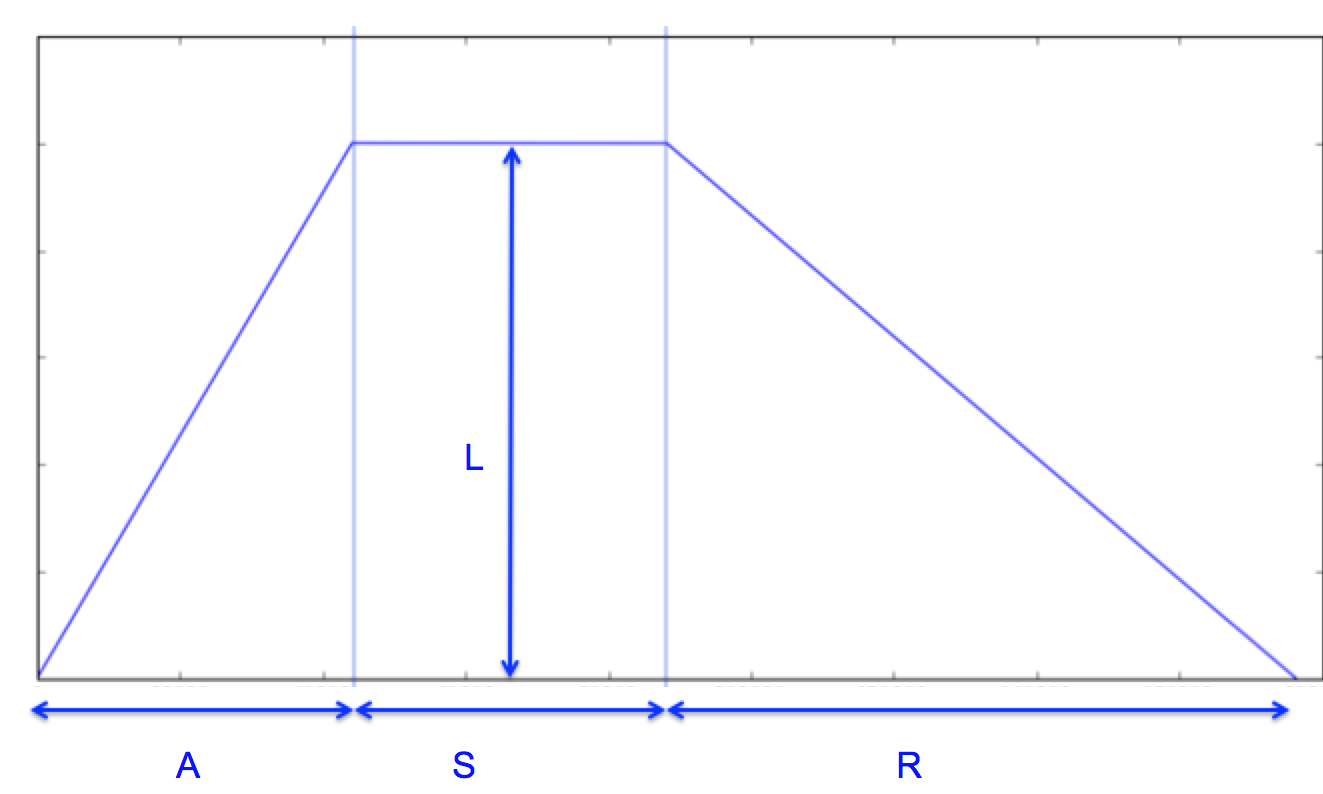
\includegraphics[width=2.5in]{Pictures/ASR.png}
%  \centering
%  \caption{\label{AmpEnv} {\it The ASR Amplitude Envelope}}
%  \centering
%  \end{figure}

\begin{figure*}[ht]
  \center
  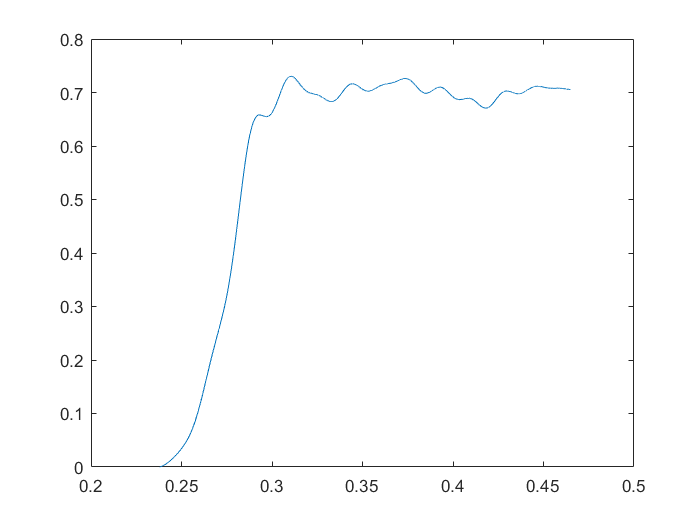
\includegraphics[width=3in]{Pictures/Attack_Env.png}
  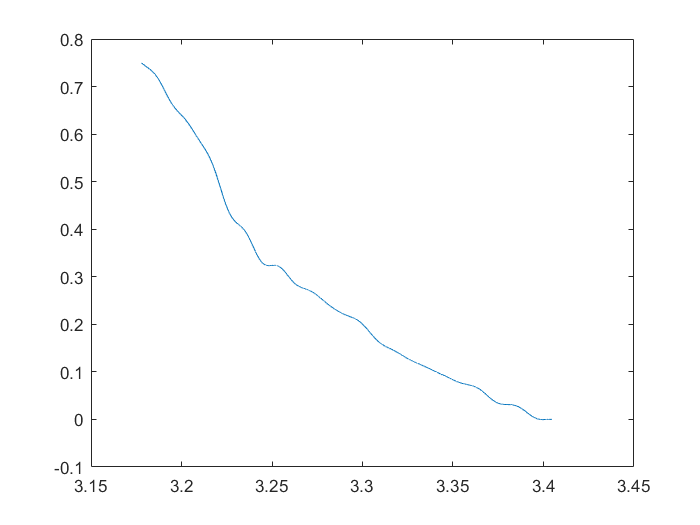
\includegraphics[width=3in]{Pictures/Release_Env.png}
  \caption{\label{AttRel} {\it Attack and Release Multipliers}}
  \end{figure*}

\begin{itemize}
\item Attack: The attack of a note is the event that triggers the onset
of the note. For example, the attack of a saxophone would be the sound of the pick
hitting the string, while the attack of a saxophone would be the sound of the tongue
hitting the reed.

\item Sustain: The sustain of a sound characterizes the way that the amplitude of
a note changes as it is held out. For a guitar, the amplitude decays as the vibration
energy of the string gradually diminishes. For the saxophone, however, the amplitude
stays roughly constant as the saxophone player uses their breath
support to maintain the volume of the note.

\item Release: Just as the attack is the event that triggers the onset of
the note, the release is the corresponding event that turns the note ``off.''
For the saxophone the release is triggered by the player choking off their air,
while the release of the guitar can be heard as the sound of the player's fingers
muting the strings.
\end{itemize}

\noindent
We converted the amplitude envelope of a
guitar to that of a saxophone by using use note detection methods to determine when
the attack, sustain, and release parts of a note began
and then using multiplier
tables to scale the signal to match the desired amplitude envelope.

\begin{figure}[ht]
  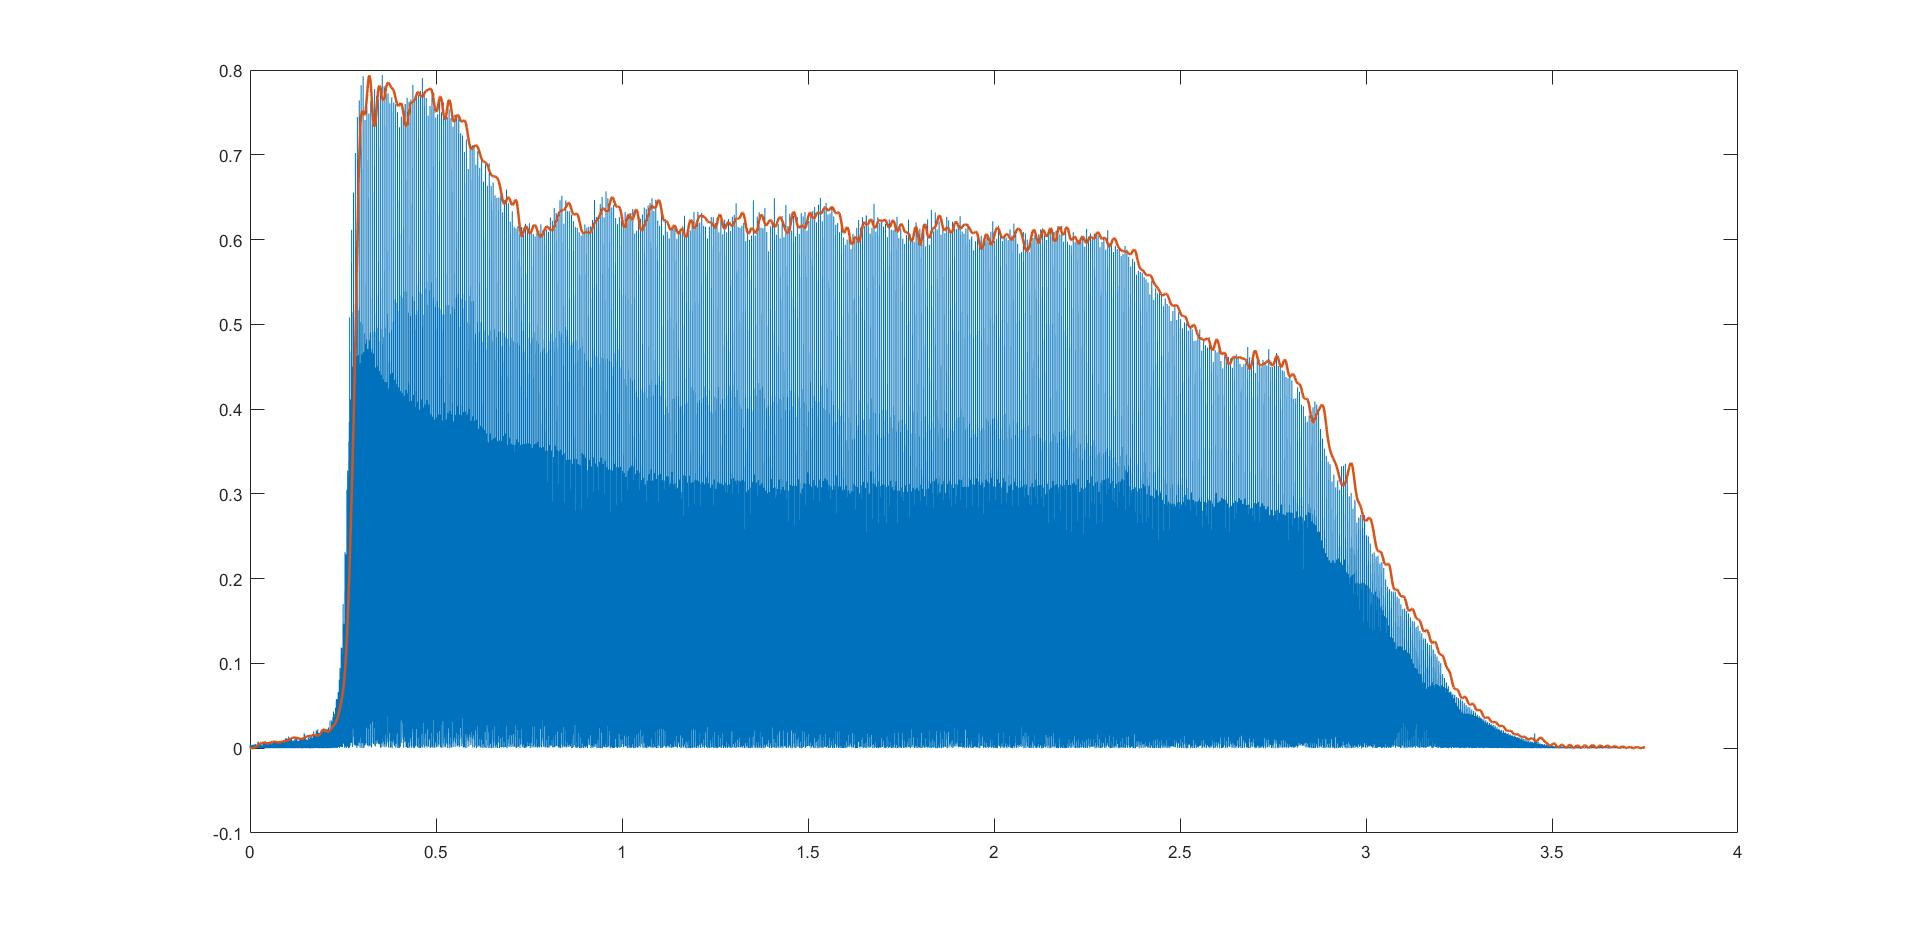
\includegraphics[width=3in]{Pictures/EnvDetection.jpg}
  \centering
  \caption{\label{SaxEnv} {\it Envelope Detection for Saxophone Sample}}
  \end{figure}

\subsection{Envelope Detection}
In order to generate the amplitude multiplier tables mentioned above,
it was first necessary to analyze saxophone and guitar samples off-line
to characterize the natural amplitude envelopes of each instrument. We
implemented an envelope detection method as described in \cite{DBLP:journals/corr/Jarne17}
which consists of rectification followed by a peaking filter followed by a low pass filter.
We were then able to store the envelope values for the attack and release parts of the waveform
to be used in real-time (see Fig. \ref{AttRel}).

\begin{figure}[ht]
  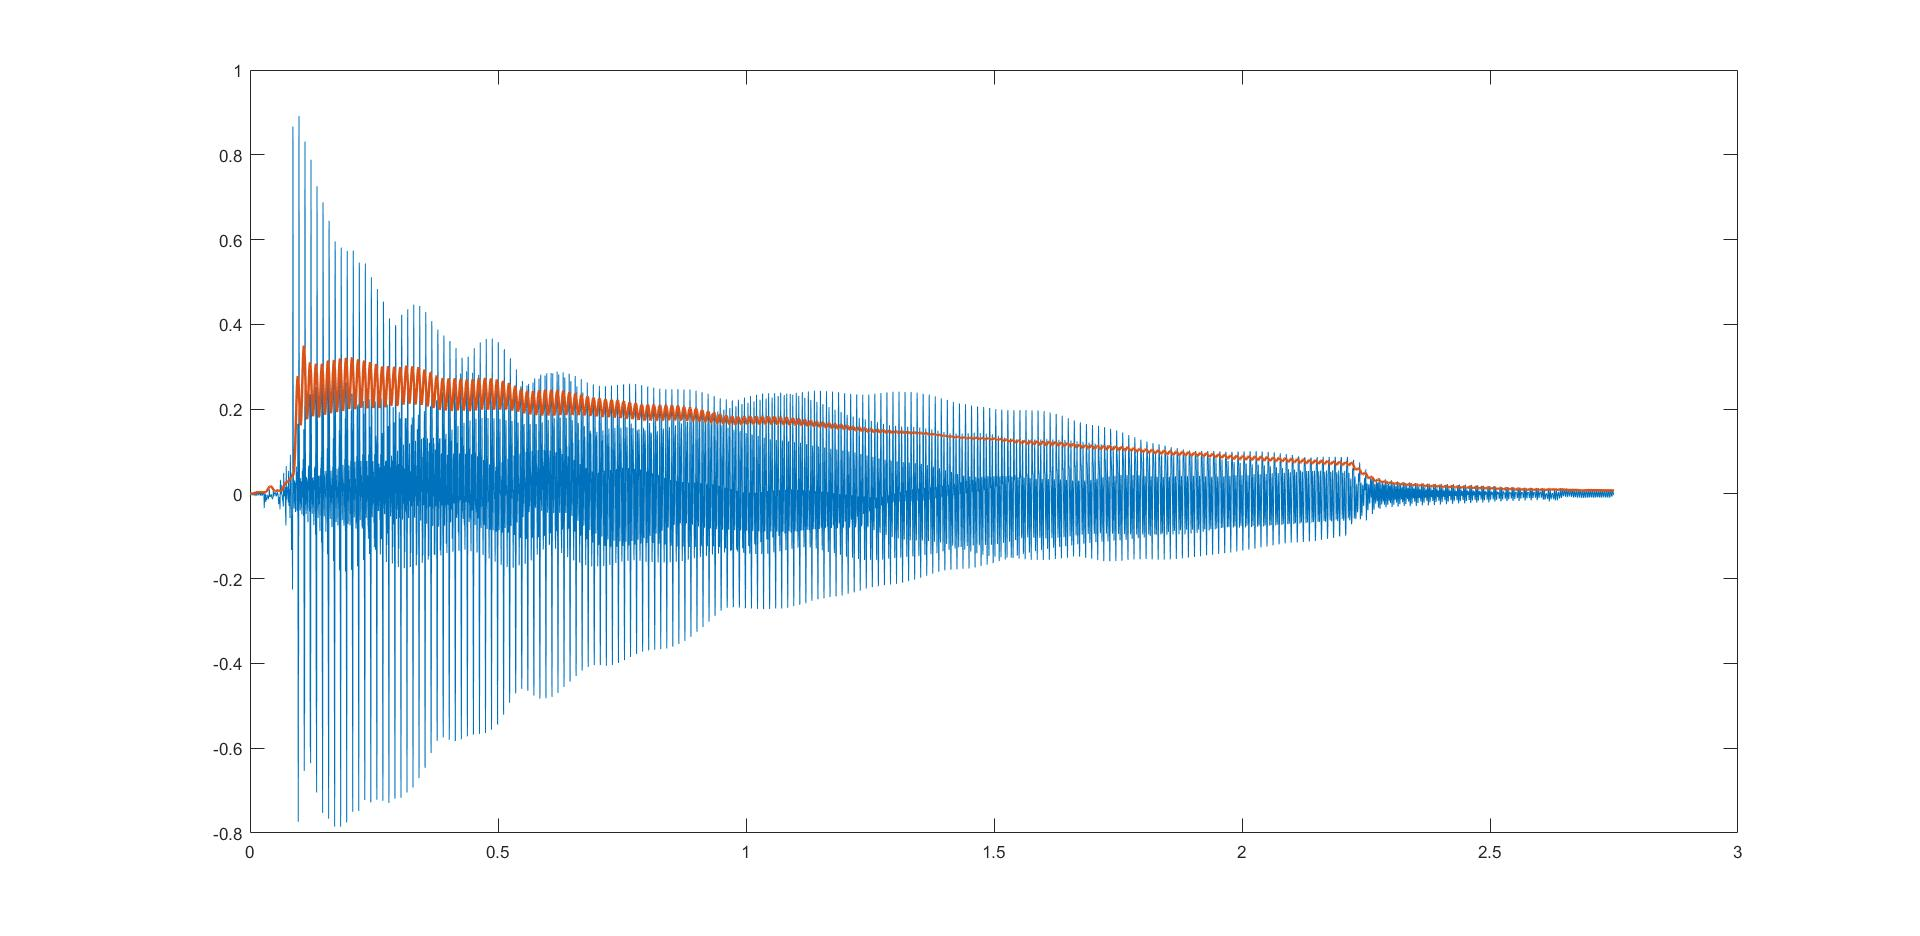
\includegraphics[width=3in]{Pictures/NoteDetect1.jpg}
  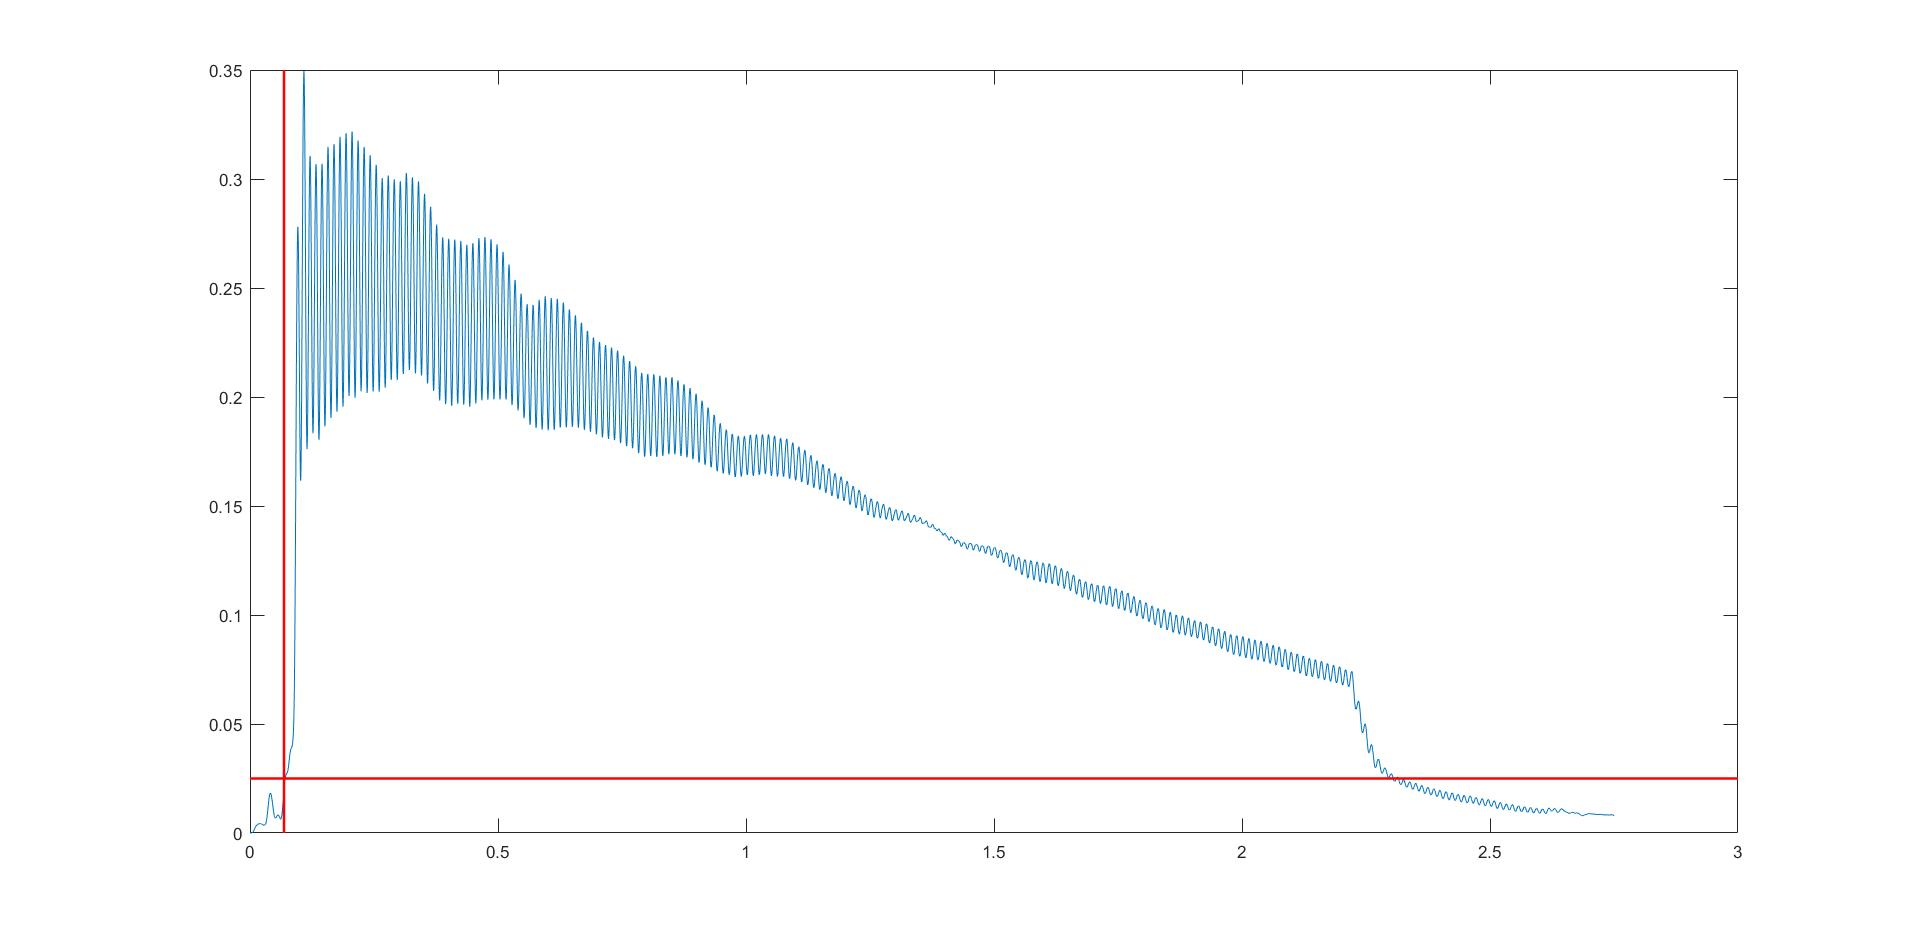
\includegraphics[width=3in]{Pictures/NoteDetect2.jpg}
  \caption{\label{Onset} {\it Note Onset Detection for Guitar Sample}}
  \centering
  \end{figure}

\subsection{Note Detection}
In order to implement the envelope modulation in real-time, it is necessary to detect
the onset and offset of every note, and use those to trigger the attack
and release multipliers. Following the process outlined in \cite{NoteOnset}
we first implemented a short window peaking filter, and then used a threshold
to determine when a new note had begun (see Fig. \ref{Onset}). Using the same method,
but with a different threshold, we were able to detect the ends of notes as well.
The issue with this method, was that if a note was already being sustained while
the next note was played, the algorithm would not be able to detect the onset of
the new note. To remedy this, we added another method of note detection: during
the sustain part of the waveform, if the output of the peaking filter was some
threshold above the average of the peaking filter window, we consider that a new
note, and thus trigger the attack envelope modulation.

\begin{figure}[ht]
  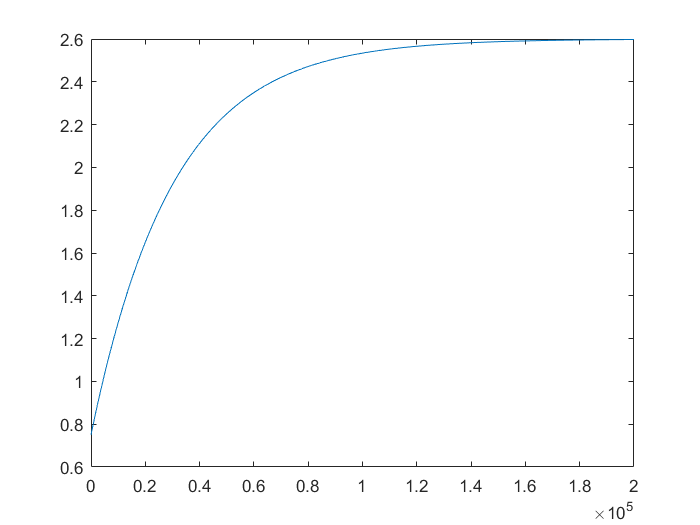
\includegraphics[width=3in]{Pictures/Sustain_Env.png}
  \centering
  \caption{\label{Sustain} {\it Sustain Envelope}}
  \centering
  \end{figure}

\subsection{Sustain}
Finding a transfer function for the sustain part of the waveform proved
to be somewhat more difficult, because unlike the attack and release,
the sustain can last for an indeterminate amount of time - as long as
the player holds the note. As such, our sustain transfer function needed
to be able to operate over an arbitrarily long signal without losing
stability. In order to meet these demands, we model the guitar sustain
as an exponential decay, and the saxophone sustain as being roughly flat.
Therefore, in order to obtain the flat response from the exponential decay,
we need to multiply the signal by an exponentially increasing function (see Fig.\ref{Sustain}).
Along with giving our sound a much more saxophone-like sustain, the advantage of
modeling the sustain in this way is that the transfer function approaches a
constant multiplier value as the sustain extends to be
arbitrarily long, thus ensuring stability.

\subsection {Results}
Ultimately, the amplitude envelopes worked as expected for all three parts
of the waveform,  creating the smooth attack that listeners expect from the
saxophone, and maintaining a roughly flat sustain while allowing the performer
some expressiveness. The note detection algorithm
worked reasonably well for single notes, but even with the enhanced note detection
scheme described above, had difficulty detecting every new note in a multi-note melody,
particularly if notes were played very quickly in succession, resulting in a slightly
``choppy'' sound. An additional improvement would be to make the threshold values more robust,
perhaps by comparing to a noise floor, rather than simply using hard-coded values.
Fig. \ref{Result} shows input and output waveforms of a single guitar note passed through
the real-time system.

\begin{figure}[ht]
  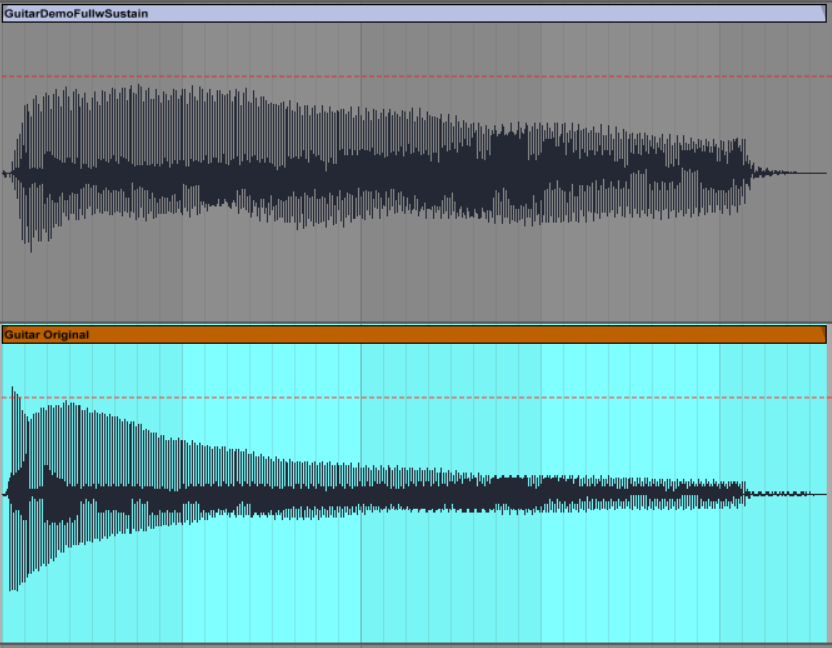
\includegraphics[width=3in]{Pictures/Final_pic.PNG}
  \centering
  \caption{\label{Result} {\it Amplitude Envelope Results: Guitar Input (below), notGuitar Output (above)}}
  \centering
  \end{figure}

\section{Future Improvements}
Our system is currently trained to be used for one note at a time,
which limits the number of things that a guitar player can do with
it. Even though saxophones technically cannot play chords, extending
the system so the user can play a chord similar to a 
saxophone ensemble would be interesting and useful.
However, this feature would require a multi-note frequency detection
algorithm, requiring more computation power.
\newline\newline
In theory the system could be extended to work not only for guitar
to saxophone, but with any melodic instrument as the input or output.
Examples would include trumpet, violin, flute, etc.. This would
require more off-line training to identify the frequency and
amplitude characteristics of each instrument. Another aspect that would enhance the user experience
would be to make the system be adaptable for users' desired control.
For example, the system could allow for the user to vary the timbre intensity
and/or have a foot pedal to control sustain length.

\section{Documentation of Real-Time System}
A video demonstration of the notGuitar system working in
real-time can be found here: \url{https://www.youtube.com/watch?v=0Gk7cZHvSLI&feature=youtu.be}.

\section{Acknowledgments}
Many thanks to Richard Leahy and Antonio Ortega for guidance and support.

%\newpage
\nocite{*}
\bibliographystyle{IEEEbib}
\bibliography{references} % requires file DAFx19_tmpl.bib

\end{document}
